\documentclass{article}
\usepackage{afterpage}
\usepackage{amsmath}
\usepackage{amssymb}
\usepackage{bbm}
\usepackage[legalpaper,margin=2cm,top=2cm,bottom=2cm]{geometry}
%\usepackage[legalpaper]{geometry}
\usepackage{graphicx}
\usepackage[utf8]{inputenc}
\usepackage[T1, T2A]{fontenc}
\usepackage[english,russian]{babel}
\usepackage{pdflscape}

\bibliographystyle{unsrt}

\DeclareMathOperator{\diag}{diag}
\DeclareMathOperator{\Arg}{Arg}

\newcommand{\bra}{\langle}
\newcommand{\ket}{\rangle} 

\title{Некоторые сюжеты о топологических изоляторах}
\author{Anikin Evgeny, 128}

\begin{document}
    \maketitle
    \subsection{Модель сильной связи для топологического изолятора}
Можно написать эквивалентный гамильтониан сильной связи. Блок
для одной компоненты спина будет иметь следующий вид (для простоты предполагается симметрия
зон):
\begin{equation}
    \label{BHZ}
    H = \left(\begin{matrix}
            \xi + \frac{1}{m}(2 - \cos{p_x} - \cos{p_y}) & 2t(\sin{p_x} - i\sin{p_y})   \\
            2t(\sin{p_x} + i\sin{p_y}) & - \xi - \frac{1}{m}(2 - \cos{p_x} - \cos{p_y}) \\
        \end{matrix}\right)
\end{equation}
Спектр этого гамильтониана несложно вычислить:
\begin{equation}
    E_p^2 = (\xi + \frac{1}{m}(2 - \cos{p_x} - \cos{p_y}))^2 + 4t^2(\sin^2{p_x} + \sin^2{p_y})
\end{equation}
Как видно, гамильтониан описывает две симметричные зоны, щель между которыми равна $2|\xi|$. 
При малых $k$ $E_p^2 = \xi^2 + (4t^2 + \xi/m)k^2$, то есть спектр дираковский.

В координатном (решёточном) представлении гамильтониан выглядит так:
\begin{multline}
    \label{BHZ_tight_binding}
    H_{\mathrm{lattice}} = \sum_{mn} \left\{
        a_{mn}^\dagger\left( \left(\xi + \frac{2}{m}\right) a_{mn}
                 -\frac{1}{2m}(a_{m+1,n} + a_{m-1,n} + a_{m,n+1} + a_{m,n-1})\right)\right. \\
        -it a_{mn}^\dagger(b_{m+1,n} -b_{m-1,n} - i(b_{m,n+1} - b_{m,n-1}))\\
        -it b_{mn}^\dagger(a_{m+1,n} -a_{m-1,n} + i(a_{m,n+1} - a_{m,n-1}))\\
        -\left. b_{mn}^\dagger\left( \left(\xi + \frac{2}{m}\right) b_{mn}
                 -\frac{1}{2m}(b_{m+1,n} + b_{m-1,n} + b_{m,n+1} + b_{m,n-1})\right) \right\}
\end{multline}
Здесь $a_{mn}$, $b_{mn}$ --- операторы уничтожения состояний двух зон 
соответственно на узле $(m,n)$. Непосредственно обобщая этот решёточный гамильтониан, можно
рассматривать решётку конечного размера, добавлять примеси и так далее. 

    \section{Точечная примесь}
Гамильтониан простейшего топологического изолятора может быть записан в виде
\begin{equation}
    \label{BHZ}
    H = \left(\begin{matrix}
            \xi + \frac{1}{m}(2 - \cos{p_x} - \cos{p_y}) & 2t(\sin{p_x} - i\sin{p_y})   \\
            2t(\sin{p_x} + i\sin{p_y}) & - \xi - \frac{1}{m}(2 - \cos{p_x} - \cos{p_y}) \\
        \end{matrix}\right)
\end{equation}
Уровни энергии ---
\begin{equation}
    E_p^2 = (\xi + \frac{1}{m}(2 - \cos{p_x} - \cos{p_y}))^2 + 4t^2(\sin^2{p_x} + \sin^2{p_y})
\end{equation}
Если перейти из импульсного представления в координатное, то он превратится в гамильтониан
сильной связи. Гамильтониан примеси тогда можно записать в виде
\begin{equation}
    V = \Delta E (a_{00}^\dagger a_{00} + b_{00}^\dagger b_{00})
\end{equation}
\subsection{Энергия связанных состояний}
Связанные состояния даются уравнением
\begin{equation}    
    \det{\left[\mathbbm{1} - \Delta E \int \frac{d^2 p}{(2\pi)^2} 
            \frac{\omega + \hat{H}}{\omega^2 - E_p^2}\right]} = 1
\end{equation}
В последнем интеграле (от матрицы) недиагональные члены из--за симметрии обращаются в ноль.
Таким образом, связанные состояния сводятся к уравнениям
\begin{equation}
    \label{integrals}
    \left[
    \begin{split}
        &\int \frac{d^2 p}{(2\pi)^2} 
            \frac{\omega + \xi + \frac{1}{m}(2 - \cos{p_x} - \cos{p_y})}
                 {\omega^2 - E_p^2} = \frac{1}{\Delta E},\\
        &\int \frac{d^2 p}{(2\pi)^2} 
            \frac{-\omega + \xi + \frac{1}{m}(2 - \cos{p_x} - \cos{p_y})}
                 {\omega^2 - E_p^2} = -\frac{1}{\Delta E},
    \end{split}
    \right.
\end{equation}
Эти интегралы можно взять приближённо в круге небольшого радиуса $p_{\mathrm{max}}$,
если учесть, что при малых $p$ спектр близок к 
коническому. После интегрирования получается
\begin{equation}
    G(\omega,0,0)_{11} = -\frac{1}{8\pi}\frac{1}{m(4t^2 + \frac{\xi}{m})}
        \left[ p_{\mathrm{max}}^2 + 
            \left(2m(\omega+\xi) - \frac{\xi^2 - \omega^2}{4t^2 + \frac{\xi}{m}}\right) 
                \log{\left(1 + \frac{\left(4t^2 + \frac{\xi}{m}\right)p_{\mathrm{max}}^2}
                                    {\xi^2 - \omega^2}\right)}\right]
\end{equation}
Конечно, интегралы из \eqref{integrals} можно взять численно. Для 
$\xi, m, t = -0.03, 0.1, 0.5$ компоненты функции Грина изображены на графике.

\begin{figure}[h]
    \centering
    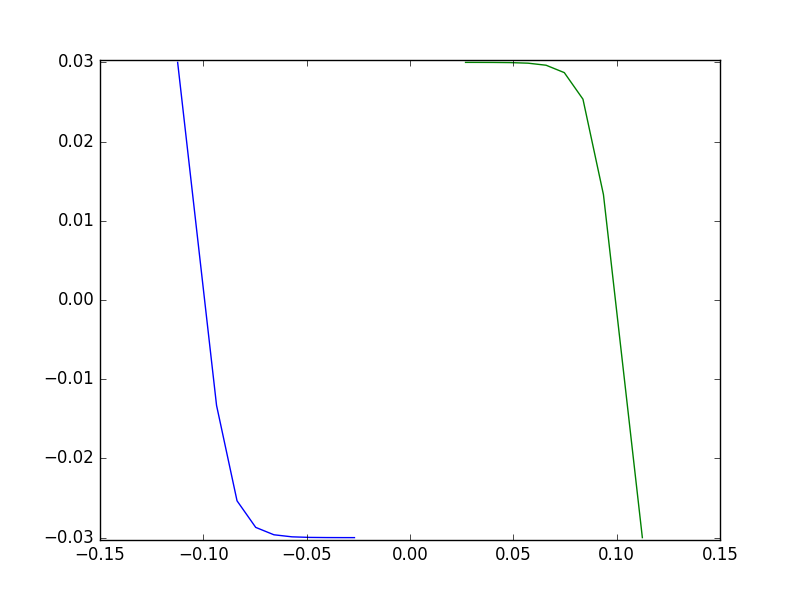
\includegraphics[width=0.8\linewidth]{impurity_levels.png}
    \caption{
            На графике показаны уровни энергии связанных состояний на точечной примеси. 
            По оси абсцисс отложена обратная глубина ямы, $\Delta E^{-1}$. <<Хвосты>>
            обоих графиков должны быть продолжены до бесконечности, у синего графика ---
            вправо снизу, у зелёного --- влево сверху. Видно,
            что при бесконечной глубине ямы имеются два слабо связанных состояния.
            }
\end{figure}

Вычисление выше показывает, что происходит на краях этого графика. А именно, ``хвосты'' 
функций Грина растут логарифмически до бесконечности.
Таким образом, для малых $\Delta E < 0$ появляется одно связанное состояние около 
зоны проводимости. При дальнейшем росте возмущения появляется состояние около валентной зоны.

\subsection{Волновые функции}
Волновые функции даются компонентами свободной
функции Грина:
\begin{equation}
    \Psi_{\alpha, i}(x) = G_0(x)_{\alpha i}
\end{equation}
Здесь $\alpha$ --- ``спинорный'' индекс, а $i$ --- индекс, соответствующий номеру волновой 
функции.

Функция Грина --- 
\begin{equation}
    G_0(x) = \int \frac{d^2 p}{(2\pi)^2} 
            \frac{\omega + \hat{H}}{\omega^2 - E_p^2} e^{ipx}
\end{equation}
Их можно вычислить с помощью формального трюка. Определим новую функцию
$F(x,y)$:
\begin{equation}
    F(x,y) = \equiv \int \frac{d^2 p}{(2\pi)^2} 
            \frac{e^{ip_x x + ip_y y}}{\omega^2 - E_p^2} 
\end{equation}
Несложно понять, что компоненты функций Грина выражаются (точными соотношениями)
 через $F(x,y)$. А именно,
\begin{equation}
    \label{differences}
    \begin{split}
        G_{11} & = (\omega + \xi) F(x,y) - 
            \frac{1}{m}(F(x+1,y) + F(x-1,y) + F(x,y+1) + F(x, y-1) - 4F(x,y))\\
        G_{21} & = -it(F(x+1,y) - F(x-1,y)) + t(F(x,y+1) - F(x,y-1))
    \end{split}
\end{equation}
С другой стороны, $F(x,y)$ может быть вычислена приближённо. Если разложить 
выражение в знаменателе около $p = 0$ и распространить интегрирование до $\infty$, то получится
сходящийся и берущийся интеграл.
\begin{equation}
    F(x,y) \approx -\int \frac{p\,dp\,d\cos{\theta}}{(2\pi)^2} 
        \frac{e^{ipr\cos{\theta}}}{\xi^2 - \omega^2 - (4t^2 + \frac{\xi}{m})p^2} = 
        -\frac{1}{2\pi} \frac{1}{4t^2 + \frac{\xi}{m}}
        K_0 \left(\sqrt{\frac{\xi^2 - \omega^2}{4t^2 + \frac{\xi}{m}}}R \right)
\end{equation}
Разности \eqref{differences} можно аппроксимировать производными. Пользуясь тем, что
$K_0(x)$ --- решение модифицированного уравнения Бесселя, получим 
\begin{equation}
    \begin{split}
        G_{11} & = -\frac{1}{2\pi} \frac{1}{4t^2 + \frac{\xi}{m}}
        \left( \omega + \xi - \frac{1}{m} \frac{\xi^2 - \omega^2}{4t^2 + \frac{\xi}{m}} \right)
        K_0 \left(\sqrt{\frac{\xi^2 - \omega^2}{4t^2 + \frac{\xi}{m}}}R \right)\\
        G_{21} & = \frac{it}{\pi} \sqrt{\frac{\xi^2 - \omega^2}
                                     {(4t^2 + \frac{\xi}{m})^{3}}}
        K_0' \left(\sqrt{\frac{\xi^2 - \omega^2}{4t^2 + \frac{\xi}{m}}}R \right)e^{i\theta}
    \end{split}
\end{equation}
%Найдём момент импульса найденных состояний. Оператор полного момента имеет вид
%\begin{equation}
%    J_z = x p_y - y p_x + \frac{1}{2}\sigma_z
%\end{equation}
%Несложно понять, что у двух найденных состояний полный момент равен $\pm \frac{1}{2}$.
%
%Интересно также найти магнитный момент. Оператор магнитного момента ---
%\begin{equation}
%    m_z = \frac{e}{2c}(x v_y - y v_x) + \frac{e}{2m_0c} \sigma_z
%\end{equation}
%Операторы скорости в низшем порядке по импульсам ---
%\begin{equation}
%    \begin{split}
%        v_x & = \begin{pmatrix} 
%                -\frac{i}{m} \partial_ x & 2t \\
%                2t & \frac{i}{m}\partial_x
%              \end{pmatrix} \\
%        v_y & = \begin{pmatrix} 
%                -\frac{i}{m} \partial_y & -2it \\
%                2it & \frac{i}{m}\partial_y
%              \end{pmatrix} \\
%    \end{split}
%\end{equation}
%Таким образом,
%\begin{equation}
%    m_z = \frac{e}{2mc}
%            \begin{pmatrix}
%               l_z & -2imt\cdot re^{-i\theta} \\
%               2imt\cdot r e^{i\theta} & -l_z
%            \end{pmatrix} + 
%          \frac{e}{2m_0c} \sigma_z
%\end{equation}

    \section{Спин--орбитальное взаимодейтвие в приближении сильной связи}
Необходимым ``ингредиентом'' для топологических изоляторов является спин--орбитальное 
взаимодействие. Экспериментальная реализация \cite{Bernevig2006, Konig2007} двумерного топологического изолятора ---
квантовая яма CdTe--HgTe--CdTe, составляющие которой --- узкозонные полупроводники с 
сильным спин--орбитальным расщеплением. Для их описания давно применяются
гамильтонианы Латтинжера и Кейна (\cite{Luttinger1956,Kane1957}). Однако эти гамильтонианы
выводятся из симметрийных соображений в $k\cdot p$ методе и, следовательно,
дают спектр только в центре зоны Бриллюэна, а также не слишком интуитивно понятны.

Мы построили простую модель сильной связи, аналогичную модели Кейна, 
учитывающую валентную $p$--зону и $s$--зону проводимости. Как показано, она переходит
в модель Кейна при малых $k$. Также она даёт возможность найти спектр во всей зоне 
Бриллюэна, а также интуитивно понятным образом описать одиночные примеси, границы образца,
резкие изменения параметров и прочее.

Модель представляет из себя 
кубическую решётку из атомов, на каждом из которых ``сидят'' состояния
с $p_x$--, $p_y$--, $p_z$-- и $s$--орбиталями и двумя 
возможными проекцими спина. В модели учитывались перекрытия
орбиталей соседних атомов, а также внутриатомное спин--орбитальное взаимодействие.
В литературе утверждается, что эффекты от межатомного спин--орбитального 
взаимодействия пренебрежимо малы.

Для написания
спин--орбитального гамильтониана $p$--зоны необходимо перейти к состояниям с определённым
полным моментом. Эти состояния выражаются через $p_x$, $p_y$, $p_z$ орбитали следующим образом:
\begin{equation}
	\label{transform1}
	\begin{gathered}
        \Psi_{\frac{3}{2},\frac{3}{2}} = \frac{X + iY}{\sqrt{2}}\alpha\\
        \Psi_{\frac{3}{2}, \frac{1}{2}} = \sqrt{\frac{1}{3}}\frac{X + iY}{\sqrt{2}}\beta -
                                         \sqrt{\frac{2}{3}} Z\alpha\\
        \Psi_{\frac{3}{2}, -\frac{1}{2}} = -\sqrt{\frac{1}{3}}\frac{X - iY}{\sqrt{2}}\alpha -
                                         \sqrt{\frac{2}{3}} Z\beta\\
        \Psi_{\frac{3}{2},-\frac{3}{2}} = -\frac{X - iY}{\sqrt{2}}\beta
	\end{gathered}
\end{equation}
\begin{equation}
	\label{transform2}
	\begin{gathered}
        \Psi_{\frac{1}{2}, \frac{1}{2}} = \sqrt{\frac{2}{3}}\frac{X + iY}{\sqrt{2}}\beta +
                                         \sqrt{\frac{1}{3}} Z\alpha\\
        \Psi_{\frac{1}{2}, -\frac{1}{2}} = -\sqrt{\frac{2}{3}}\frac{X - iY}{\sqrt{2}}\alpha-
                                         \sqrt{\frac{1}{3}} Z\beta\\
	\end{gathered}
\end{equation}
Здесь $X,Y,Z$ --- атомные орбитали, $\alpha,\beta$ --- состояния со спином вверх и вниз.

Как хорошо известно, в атоме гамильтониан спин--орбитального взаимодейстия имеет вид
\begin{equation}
    H_{\mathrm{SO}} =  A(\vec{S}, \vec{L}) = \frac{A}{2}(J^2 - L^2 - S^2)
\end{equation}
Если орбитальный момент фиксирован, то энергия определяется полным моментом. Таким образом,
спин--орбитальное взаимодействие приводит к расщеплению состояний с моментами $\frac32$ и
$\frac12$.

Пусть матричные элементы перекрытия $p$-- орбиталей --- $t_\parallel$ и $t_\perp$. Тогда
несложно показать, что гамильтониан тяжёлых и лёгких дырок в импульсном представлении ---
\begin{equation}
    \begin{gathered}
    H_v = \begin{bmatrix}
            H_l & H_r
        \end{bmatrix},\\
    H_l = 
    \begin{pmatrix}
        (t_\parallel + t_\perp)(\cos{p_x} + \cos{p_y}) + 2t_\perp \cos{p_z} & 0 \\
        0 & \left(\frac{t_\parallel}{3} + \frac{5t_\perp}{3}\right)(\cos{p_x}+\cos{p_y})+ 
                           \left(\frac{2t_\perp}{3} + \frac{4t_\parallel}{3}\right)\cos{p_z} \\
        -\frac{1}{\sqrt{3}}(t_\parallel - t_\perp)(\cos{p_x} - \cos_{p_y}) & 0 \\
        0 & -\frac{1}{\sqrt{3}}(t_\parallel - t_\perp)(\cos{p_x} - \cos_{p_y}) 
    \end{pmatrix}\\
    H_r = 
    \begin{pmatrix}
        -\frac{1}{\sqrt{3}}(t_\parallel - t_\perp)(\cos{p_x} - \cos_{p_y}) & 0 \\
        0 & -\frac{1}{\sqrt{3}}(t_\parallel - t_\perp)(\cos{p_x} - \cos_{p_y})\\
       \left(\frac{t_\parallel}{3} + \frac{5t_\perp}{3}\right)(\cos{p_x} + \cos{p_y}) + 
                    \left(\frac{2t_\perp}{3} + \frac{4t_\parallel}{3}\right)\cos{p_z} & 0 \\
        0 & (t_\parallel + t_\perp)(\cos{p_x} + \cos{p_y}) + 2t_\perp \cos{p_z}
    \end{pmatrix}
    \end{gathered}
\end{equation}
Э разумеется,ту матрицу можно разложить около нуля. Тогда получится хорошо известный 
гамильтониан Латтинжера \cite{Luttinger1956}:
\begin{equation}
    H_v = -\left(\gamma_1 + \frac{5}{2}\gamma_2\right) k^2 + 
        2\gamma_2(k_x^2J_x^2 + k_y^2J_y^2 + k_z^2J_z^2),
\end{equation}
где $J_i$ --- операторы момента для спина $\frac{3}{2}$, $\gamma_1 = \frac13 t_\parallel$,
$\gamma_2 = \frac16(t_\parallel - t_\perp)$, $\gamma_3 = 0$ (последнее слагаемое 
из гамильтониана Латтинжера опущено).

Теперь учтём перекрытие с $s$--зоной. Оно задаётся матрицей
\begin{equation}
    T = P\begin{pmatrix}
            -\frac{1}{\sqrt{2}}(\sin{p_x} + i\sin{p_y}) & \sqrt{\frac{2}{3}}\sin{p_z} &
             \frac{1}{\sqrt{6}}(\sin{p_x} - i\sin{p_y}) & 0 \\  
            0 & -\frac{1}{\sqrt{6}}(\sin{p_x} + i\sin{p_y}) & 
            \sqrt{\frac{2}{3}}\sin{p_z} & \frac{1}{\sqrt{2}}(\sin{p_x} - i\sin{p_y}),
         \end{pmatrix},
\end{equation}
где $P = 2i\langle s(x+e_x) | \hat{H} | p_x(x)\rangle$. Наконец, гамильтониан самой 
$s$--зоны можно записать как 
\begin{equation}
    H_c = (E_s + \frac{1}{m_s}(3 - \cos{p_x} - \cos{p_y} - \cos{p_z}))I_{2\times2}
\end{equation}
Состояниями с полным моментом $\frac{1}{2}$ 
можно пренебречь, если спин--орбитальное взаимодейтвие велико.
Таким образом мы получаем гамильтониан с учётом $s$--зоны проводимости, зон тяжёлых и
лёгких дырок в виде
\begin{equation}
    \label{hfull}
    H_{\mathrm{full}} = \begin{pmatrix}
                            H_c & T \\
                            T^\dagger & H_v
                        \end{pmatrix},
\end{equation}
где $H_c, T, H_v$ определены выше. Линеаризуя его, мы получим гамильтониан модели Кейна
\cite{Kane1957}.

Спектр такой модели не может быть найден аналитически для произвольных $k_x, k_y, k_z$. Однако
ветви спектра можно легко найти, если, например, $k_x = k_y = 0$. Для этого случая 
спектр в окрестности центра зоны Бриллюэна изображён на рисунке. Как видно, он состоит
из трёх ветвей: одной электронной ветви и двух ветвей дырок, тяжёлых и лёгких.

\begin{figure}
    \centering
    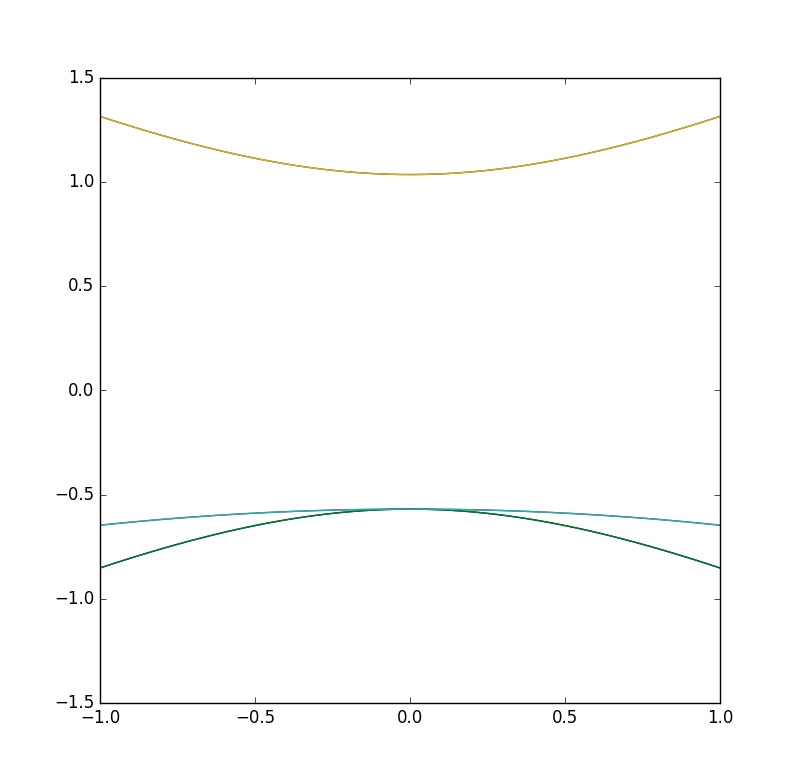
\includegraphics[width=0.6\linewidth]{cdte.png}
    \caption{На графике изображены ветви спектра CdTe в модели Кейна для параметров
             из \cite{Novik2005}. По оси абсцисс отложен волновой вектор в $\mathrm{nm}^{-1}$,
             по оси орбинат --- энергия в eV.}
\end{figure}

Таким образом, простая модель сильной связи воспроизводит известные свойства 
полупроводников со спин--орбитальным взаимодействием.

%\begin{equation}
%\scalebox{0.6}{%
%$
%H_v = \begin{pmatrix}
%       (t_\parallel + t_\perp)(\cos{p_x} + \cos{p_y}) + 2t\perp \cos{p_z} & 0 &
%       -\frac{1}{\sqrt{3}}(t_\parallel - t_\perp)(\cos{p_x} - \cos_{p_y}) & 0 \\
%
%       0 & \left(\frac{t_\parallel}{3} + \frac{5t_\perp}{3}\right)(\cos{p_x} + \cos{p_y}) + 
%                   \left(\frac{2t_\perp}{3} + \frac{4t_\parallel}{3}\right)\cos{p_z} & 
%       0 & -\frac{1}{\sqrt{3}}(t_\parallel - t_\perp)(\cos{p_x} - \cos_{p_y})\\
%       -\frac{1}{\sqrt{3}}(t_\parallel - t_\perp)(\cos{p_x} - \cos_{p_y}) & 0 &
%      \left(\frac{t_\parallel}{3} + \frac{5t_\perp}{3}\right)(\cos{p_x} + \cos{p_y}) + 
%                   \left(\frac{2t_\perp}{3} + \frac{4t_\parallel}{3}\right)\cos{p_z} & 0 \\
%       0 & -\frac{1}{\sqrt{3}}(t_\parallel - t_\perp)(\cos{p_x} - \cos_{p_y}) & 
%       0 & (t_\parallel + t_\perp)(\cos{p_x} + \cos{p_y}) + 2t\perp \cos{p_z}
%      \end{pmatrix}
%$
%}
%\end{equation}


%Гамильтониан имеет вид
%\begin{multline}
%   \label{well_model_ham}
%   H  = \sum_{m,n} (E_s + 4t_s) s_{mn}^{\dagger} s_{mn} - t_s s_{mn}^{\dagger}
%                          (s_{m+1,n} + s_{m-1,n} + s_{m,n+1} + s_{m,n-1}) \\
%          + t_{sp} s_{mn}^{\dagger} (-p_{m+1,n}^x + p_{m-1,n}^x - p^y_{m,n+1} + p^y_{m,n-1})
%                                                                + \mathrm{h.c.}  \\
%          + (p_{mn}^x)^{\dagger}(t_{\parallel}(p_{m+1,n}^x + p_{m-1,n}^x) +
%                                 t_{\perp} (p^x_{m,n+1} + p^x_{m,n-1})) \\
%          + (p_{mn}^x)^{\dagger}(t_{\perp}(p_{m+1,n}^y + p_{m-1,n}^y) +
%                                 t_{\parallel} (p^y_{m,n+1} + p^y_{m,n-1})) \\
%          + (p_{mn}^z)^{\dagger} t_3 (p_{m+1,n}^z + p_{m-1,n}^z +
%                                p^z_{m,n+1} + p^z_{m,n-1}) \\
%          -\frac{E_{SO}}{3}
%                \begin{matrix}
%                    \left(\begin{matrix}
%                        p_x^\dagger & p_y^\dagger & p_z^\dagger
%                    \end{matrix}\right) \\
%                    \\
%                    \\
%                \end{matrix}
%        		\left(\begin{matrix}
%        			1 & i & -1 \\
%        			-i & 1 & i \\
%        			-1 & -i & 1
%        		\end{matrix} \right)
%                \left(\begin{matrix}
%                    p_x \\ 
%                    p_y \\
%                    p_z
%                \end{matrix}\right) + \\
%        + \text{всё то же самое с переворотом проекции спина}
%\end{multline}
%
%Тогда спин--орбитальный гамильтониан запишется так:
%\begin{equation}
%	H_{\mathrm{full}} = -\Delta E_{SO} 
%			(a_{\frac{1}{2}, \frac{1}{2}}^\dagger a_{\frac{1}{2}, \frac{1}{2}} +
%			a_{\frac{1}{2}, -\frac{1}{2}}^\dagger a_{\frac{1}{2}, -\frac{1}{2}})
%\end{equation}
%После простого преобразования получается последнее слагаемое в \eqref{well_model_ham}.

    \section{Реконструкция края}
В данном разделе рассматривается реконструкция края (аналогично \cite{Wang2017}) 
в модели сильной связи из \cite{Bernevig2006}.

Реконструкцией края (edge reconstruction) называется следующее явление.

    \newpage
    \bibliography{literature}
\end{document}
